\documentclass{thesisSWUFE}

% 封面信息。
\covertitle{\shortstack[c]{宽松风险平价在全球 ETF\\资产配置中的改进与实证研究}}
\covercollege{特拉华数据科学学院}
\covermajor{金融数学（金融服务与量化分析方向）}
\coverauthor{许哲圣}
\coverstudentid{42353012}
\covergrade{2023级}
\coveradvisor{王磊}
\coverdate{2026年8月}

\graphicspath{{../../results/figures/}}

\hypersetup{
  pdftitle={宽松风险平价在全球 ETF 资产配置中的改进与实证研究},
  pdfauthor={许哲圣},
  pdfkeywords={宽松风险平价, 全球多资产配置, CVaR, ETF}
}

\setlength{\emergencystretch}{2em}
\renewcommand{\arraystretch}{1.18}

% 论文中的核心数值通过宏统一引用，以保持全文口径一致。
% generated_numbers.tex defines what the pipeline produced; fallback fills any remaining gaps.
\IfFileExists{generated_numbers.tex}{\newcommand{\evalStartDate}{2018-01-02}
\newcommand{\evalEndDate}{2026-09-11}
\newcommand{\etfCount}{30}
\newcommand{\txCostBps}{3}
\newcommand{\annualizationDays}{252}
\newcommand{\lookbackDays}{252}
\newcommand{\primaryRebalances}{445}
\newcommand{\primaryObservations}{2111}
\newcommand{\primaryCashMean}{18.02\%}
\newcommand{\primaryCashMax}{26.43\%}
\newcommand{\primaryDefensiveMean}{66.29\%}
\newcommand{\primaryAssetsUsed}{30}
\newcommand{\primarySelectionInformativeYears}{0}
\newcommand{\primaryParameterYears}{10}
\newcommand{\primaryReturnTargetDef}{$R_t=\mu_t^\mathsf{T}q_t$，即当期可行风险预算参考的预测收益}
\newcommand{\globalGrossReturn}{6.15\%}
\newcommand{\globalNetReturn}{6.09\%}
\newcommand{\globalVolatility}{3.59\%}
\newcommand{\globalMaxDD}{-6.80\%}
\newcommand{\globalMonthlyTurnover}{17.38\%}
\newcommand{\globalCostDrag}{0.07\%}
\newcommand{\globalCVaR}{0.53\%}
\newcommand{\globalSharpe}{1.664}
\newcommand{\globalSortino}{2.377}
\newcommand{\globalCalmar}{0.895}
}{}
\IfFileExists{generated_fallback.tex}{% Auto-generated fallback definitions. Do not edit by hand.
% Placeholder values compile the thesis before all pipeline outputs exist.

\providecommand{\dailEtfVol}{?}
\providecommand{\goldEtfReturn}{?}
\providecommand{\goldEtfVol}{?}
\providecommand{\silverLofReturn}{?}
\providecommand{\silverLofVol}{?}
\providecommand{\chuangyeEtfReturn}{?}
\providecommand{\chinaKoreaObs}{?}
\providecommand{\chinaKoreaReturn}{?}
\providecommand{\chinaKoreaVol}{?}
\providecommand{\kcbFiftyObs}{?}
\providecommand{\walkforwardSharpeMean}{?}
\providecommand{\walkforwardSharpeStd}{?}
\providecommand{\walkforwardSharpeMin}{?}
\providecommand{\walkforwardSharpeMax}{?}
\providecommand{\walkforwardSharpeMedian}{?}
\providecommand{\walkforwardNetreturnMean}{?}
\providecommand{\walkforwardNetreturnStd}{?}
\providecommand{\walkforwardNetreturnMin}{?}
\providecommand{\walkforwardNetreturnMax}{?}
\providecommand{\walkforwardNetreturnPFive}{?}
\providecommand{\walkforwardNetreturnPNinetyFive}{?}
\providecommand{\walkforwardMaxddMean}{?}
\providecommand{\costBreakevenImprovedVsGlobal}{?}
\providecommand{\costBreakevenGlobalVsEqual}{?}
\providecommand{\costBreakevenDefensiveVsEqual}{?}
\providecommand{\freqWeeklyNetReturn}{?}
\providecommand{\freqWeeklySharpe}{?}
\providecommand{\freqWeeklyMaxDD}{?}
\providecommand{\freqWeeklyMonthlyTurnover}{?}
\providecommand{\freqWeeklySolverFallback}{?}
\providecommand{\freqWeeklyRebalanceCount}{?}
\providecommand{\freqBiweeklyNetReturn}{?}
\providecommand{\freqBiweeklySharpe}{?}
\providecommand{\freqBiweeklyMaxDD}{?}
\providecommand{\freqBiweeklyMonthlyTurnover}{?}
\providecommand{\freqBiweeklySolverFallback}{?}
\providecommand{\freqBiweeklyRebalanceCount}{?}
\providecommand{\freqMonthlyNetReturn}{?}
\providecommand{\freqMonthlySharpe}{?}
\providecommand{\freqMonthlyMaxDD}{?}
\providecommand{\freqMonthlyMonthlyTurnover}{?}
\providecommand{\freqMonthlySolverFallback}{?}
\providecommand{\freqMonthlyRebalanceCount}{?}
\providecommand{\freqQuarterlyNetReturn}{?}
\providecommand{\freqQuarterlySharpe}{?}
\providecommand{\freqQuarterlyMaxDD}{?}
\providecommand{\freqQuarterlyMonthlyTurnover}{?}
\providecommand{\freqQuarterlySolverFallback}{?}
\providecommand{\freqQuarterlyRebalanceCount}{?}
\providecommand{\freqWeeklyMonthlyTurnoverGap}{?}
\providecommand{\improvedVolAlignedHrpNetReturn}{?}
\providecommand{\improvedVolAlignedHrpSharpe}{?}
\providecommand{\improvedVolAlignedHrpVolatility}{?}
\providecommand{\improvedVsGlobalDiff}{?}
\providecommand{\improvedVsGlobalCILow}{?}
\providecommand{\improvedVsGlobalCIHigh}{?}
\providecommand{\improvedVsGlobalPValue}{?}
\providecommand{\improvedVsGlobalSignificant}{?}
\providecommand{\improvedVsDefensiveDiff}{?}
\providecommand{\improvedVsDefensiveCILow}{?}
\providecommand{\improvedVsDefensiveCIHigh}{?}
\providecommand{\improvedVsDefensivePValue}{?}
\providecommand{\improvedVsDefensiveSignificant}{?}
\providecommand{\improvedVsEqualDiff}{?}
\providecommand{\improvedVsEqualCILow}{?}
\providecommand{\improvedVsEqualCIHigh}{?}
\providecommand{\improvedVsEqualPValue}{?}
\providecommand{\improvedVsEqualSignificant}{?}
\providecommand{\globalVsEqualDiff}{?}
\providecommand{\globalVsEqualCILow}{?}
\providecommand{\globalVsEqualCIHigh}{?}
\providecommand{\globalVsEqualPValue}{?}
\providecommand{\globalVsEqualSignificant}{?}
\providecommand{\defensiveVsEqualDiff}{?}
\providecommand{\defensiveVsEqualCILow}{?}
\providecommand{\defensiveVsEqualCIHigh}{?}
\providecommand{\defensiveVsEqualPValue}{?}
\providecommand{\defensiveVsEqualSignificant}{?}

}{}
\newcommand{\primaryCashMean}{70.23\%}
\newcommand{\primaryCashMax}{86.61\%}
\newcommand{\primaryChinaBondSharpe}{0.529}
\newcommand{\primaryRebalances}{444}
\newcommand{\primaryObservations}{2102}


\setlength{\textfloatsep}{14pt plus 2pt minus 3pt}
\setlength{\floatsep}{12pt plus 2pt minus 2pt}
\setlength{\intextsep}{12pt plus 2pt minus 2pt}
\captionsetup[figure]{font=small,labelfont=bf,labelsep=space,skip=6pt}

\newcommand{\figmaybe}[3]{
  \IfFileExists{../../results/figures/#1}{
    \begin{figure}[tbp]
      \centering
      \includegraphics[width=0.84\textwidth]{#1}
      \caption{#2}
      \label{#3}
    \end{figure}
  }{
    \begin{figure}[tbp]
      \centering
      \fbox{\parbox{0.84\textwidth}{\centering 图文件未找到：#1}}
      \caption{#2}
      \label{#3}
    \end{figure}
  }
}

\newcommand{\figwide}[3]{
  \IfFileExists{../../results/figures/#1}{
    \begin{figure}[tbp]
      \centering
      \includegraphics[width=0.93\textwidth]{#1}
      \caption{#2}
      \label{#3}
    \end{figure}
  }{
    \begin{figure}[tbp]
      \centering
      \fbox{\parbox{0.93\textwidth}{\centering 图文件未找到：#1}}
      \caption{#2}
      \label{#3}
    \end{figure}
  }
}

\newcommand{\fignarrow}[3]{
  \IfFileExists{../../results/figures/#1}{
    \begin{figure}[tbp]
      \centering
      \includegraphics[width=0.76\textwidth]{#1}
      \caption{#2}
      \label{#3}
    \end{figure}
  }{
    \begin{figure}[tbp]
      \centering
      \fbox{\parbox{0.76\textwidth}{\centering 图文件未找到：#1}}
      \caption{#2}
      \label{#3}
    \end{figure}
  }
}

% 并排双图宏：#1/#2 文件名，#3/#4 caption，#5/#6 label
\newcommand{\figpair}[6]{%
  \begin{figure}[tbp]
    \centering
    \begin{minipage}[t]{0.48\textwidth}
      \IfFileExists{../../results/figures/#1}{%
        \includegraphics[width=\linewidth]{#1}%
      }{%
        \fbox{\parbox{\linewidth}{\centering 图文件未找到：#1}}%
      }
      \captionof{figure}{#3}
      \label{#5}
    \end{minipage}\hfill
    \begin{minipage}[t]{0.48\textwidth}
      \IfFileExists{../../results/figures/#2}{%
        \includegraphics[width=\linewidth]{#2}%
      }{%
        \fbox{\parbox{\linewidth}{\centering 图文件未找到：#2}}%
      }
      \captionof{figure}{#4}
      \label{#6}
    \end{minipage}
  \end{figure}
}

\begin{document}

\makecover

\clearpage
\section*{学术声明}
本人郑重声明：所呈交的毕业论文是在指导教师指导下独立完成的研究成果。论文中引用他人已经发表或未发表的成果，均已在正文和参考文献中作出明确标注。除文中已经注明引用的内容外，本文不包含任何其他个人或集体已经发表或撰写过的研究成果。对本文研究作出重要贡献的个人和集体，均已在文中以明确方式说明。

\clearpage
\setcounter{page}{1}
\renewcommand{\abstractname}{摘要}
\begin{abstract}
长期资产配置需要在市场不确定时维持有效的风险分散。风险平价减少了模型对收益预测的依赖，但在全球多资产 ETF 资产池中落地时，仍需处理相关结构时变、等风险贡献条件非凸以及调仓成本累积等问题。

本文以 \etfCount 支中国市场可交易的全球多资产 ETF 构建统一回测框架，覆盖八类资产。评价区间为 \evalStartDate{} 至 \evalEndDate{}，无风险利率按研究约定设为零，按 243 个交易日年化，单边交易成本为 \txCostBps{} bps。主模型 Improved Convex Adaptive Global RRP 每周最后一个实际交易日调仓，取消现金组与单资产集中度上限；其余模型作为月频对照，频率差异另行检验。

主模型净年化收益为 \improvedNetReturn，年化波动率为 \improvedVolatility，夏普比率为 \improvedSharpe，Sortino 比率为 \improvedSortino，最大回撤为 \improvedMaxDD，月均换手率为 \improvedMonthlyTurnover。平均现金类 ETF 权重为 \primaryCashMean，最高为 \primaryCashMax；若使用滞后一月的中债国债收益率作为机会成本，同一组合夏普为 \primaryChinaBondSharpe。主模型未启用 CVaR 惩罚。其规格是在历史约束实验后选定的，因此结果属于探索性历史证据，不等同于未参与模型选择的独立样本外检验。

以上结论基于特定历史区间和约束设定，不构成对未来收益的预测。

\noindent\textbf{关键词：} 宽松风险平价；全球多资产配置；CVaR；换手约束；凸优化；ETF
\end{abstract}

\clearpage
\renewcommand{\abstractname}{Abstract}
\begin{abstract}
Risk parity replaces expected-return estimation with risk budgeting, which makes it theoretically more robust. In practice, applying it to a global multi-asset ETF universe introduces three problems that don't go away: time-varying correlations, the non-convexity of exact equal-risk-contribution constraints, and transaction costs that add up meaningfully at monthly rebalancing frequency.

This thesis studies \etfCount{} tradable ETFs across eight asset categories over \evalStartDate{} to \evalEndDate{}. The designated primary model, Improved Convex Adaptive Global RRP, rebalances weekly, removes cash-group and individual-asset concentration caps, and retains the other group and turnover controls. All headline metrics use zero risk-free return, 243 trading days per year and \txCostBps{} bps one-way transaction costs. Other core models are monthly comparisons, with separate frequency-only tests.

The primary model records \improvedNetReturn{} net annual return, \improvedVolatility{} annual volatility, \improvedSharpe{} Sharpe, \improvedSortino{} Sortino, \improvedMaxDD{} maximum drawdown and \improvedMonthlyTurnover{} average monthly turnover. Its average money-market ETF allocation is \primaryCashMean{}, reaching \primaryCashMax{}. Using lagged ChinaBond yields as opportunity cost yields a Sharpe of \primaryChinaBondSharpe{} for the same return path. The active CVaR penalty is zero. Specification selection followed historical constraint experiments, so prior-only rebalance inputs do not establish untouched out-of-sample model-selection evidence.

All results are conditional on this evaluation period and constraint settings. They do not predict future performance.

\noindent\textbf{Keywords:} Relaxed Risk Parity; Global Multi-Asset Allocation; CVaR; Turnover Constraint; Convex Optimization; ETF
\end{abstract}

\clearpage
\pagenumbering{gobble}
\tableofcontents
\clearpage
\pagenumbering{arabic}

\section{绪论}

\subsection{研究背景与意义}
资产配置在很大程度上决定了长期组合的风险收益特征\cite{brinson1986determinants}。与短期择时策略相比，长期资产配置更关注不同资产类别间的风险来源、回撤控制和流动性管理。保险资金、养老金和银行理财等长期资金通常需要在多年时间维度上维持稳定的风险暴露，管理难度不只在于收益水平，如何说清楚收益来自哪里、风险分散到什么程度、调仓成本是否可控，同样是实际问题。

风险平价和风险预算方法正是针对这类需求发展起来的。其核心思想不是资本金额的均匀分配，而是使不同资产对组合总风险的贡献更加均衡。这种方法对收益预测的依赖程度较低，适合构建可解释性强的长期配置框架\cite{qian2005risk,maillard2010properties}。扩展到全球 ETF 后，问题变得复杂：不同市场收盘时间不一致，海外 ETF 带汇率暴露，各标的上市时间参差不齐，商品和权益的尾部行为差异明显。交易成本和换手的累积尤其重要，月度调仓在长周期内会侵蚀相当一部分净收益。

从理论层面看，将严格等风险贡献条件改写为凸的风险预算参考问题，再以参考权重跟踪、方差、换手和资产组边界构造第二阶段问题，可以得到可验证的凸优化模型。候选族允许加入 CVaR 惩罚或上限，但公开滚动路径最终选择的候选没有启用 CVaR 惩罚。从实践层面看，以可交易 ETF 替代部分原始指数，使回测结果更接近真实组合执行，也便于评估交易成本对长期收益的影响。

\subsection{研究问题与研究思路}
本文围绕四个问题展开。宽松风险平价能否在 30 支全球 ETF 中建立风险来源清晰的配置框架？凸化后的参考权重跟踪、换手惩罚和资产组约束如何影响收益、回撤与换手率？包含 CVaR 的候选设定是否获得滚动样本外选择？HERC 等层次化基准在同一样本中表现如何，稳健性检验又能否识别结论对样本期和参数选择的依赖？

本文先梳理均值-方差、风险预算、CVaR 和层次化配置方法的理论联系，再建立可交易 ETF 资产池和统一回测标准，然后在相同研究设计下比较各模型，最后用多维度稳健性检验和过拟合诊断约束结论的适用范围。

\subsection{研究内容与章节安排}
论文分七章。第二章综述投资组合与风险预算文献。第三章给出凸优化目标和约束。第四章说明资产池、收益记账和信息时序。第五章比较主模型与对照的绩效和权重。第六章报告约束消融、自然年分解和频率实验，并区分参数选择与逐期信息使用。第七章总结结论与研究边界。

\subsection{可能的边际贡献}
本文采用可交易 ETF 和逐期可投池构建实验环境，以凸风险预算参考和凸跟踪问题生成权重。约束消融同时报告实际权重、交易成本、约束松弛量与对偶变量，使绩效差异能够对应到约束是否生效。对历史选定规格与未参与选择的样本外证据作明确区分，避免将高夏普比率直接解释为普遍优势。

\section{文献综述与理论基础}

\subsection{现代投资组合理论与估计误差}
Markowitz（1959）\cite{markowitz1959portfolio} 将组合选择表述为均值--方差优化。该框架依赖期望收益和协方差输入，而收益估计误差会被优化器放大。Michaud（1989）\cite{michaud1989enigma}、Chopra 与 Ziemba（1993）\cite{chopra1993effect} 说明了这种不稳定性；DeMiguel 等（2009）\cite{demiguel2009optimal} 进一步发现，有限样本下复杂优化未能稳定优于等权组合。

协方差估计同样影响样本外权重。Laloux 等（1999）\cite{laloux1999noise} 证明样本协方差包含大量噪声特征值，Jagannathan 与 Ma（2003）\cite{jagannathan2003risk} 说明权重约束具有隐式收缩作用。本文据此降低对收益预测的依赖，并比较样本协方差、EWMA 与 Ledoit--Wolf 收缩估计。

\subsection{风险平价与宽松风险平价}

风险平价以风险贡献衡量分散程度。Qian（2005）\cite{qian2005risk} 提出风险平价思想，Maillard 等（2010）\cite{maillard2010properties} 讨论了 ERC 组合的存在性和唯一性，Roncalli（2013）\cite{roncalli2013introduction} 将其推广为差异化风险预算。该方法减少了对收益预测的依赖，但严格风险贡献等式在叠加权重、组别和交易约束后难以稳定求解。

Gambeta 与 Kwon（2020）\cite{gambeta2020risk} 用偏离惩罚放松严格等式，允许风险预算与现实约束同时进入目标函数。Ardia 等（2018）\cite{ardia2018beyond} 也表明，受控偏离能够改善风险调整收益。本文沿用这一思路，把 CVaR、换手惩罚和资产组边界纳入同一凸优化近似。

\subsection{CVaR、交易成本与层次化基准}

Rockafellar 与 Uryasev（2000；2002）\cite{rockafellar2000optimization,rockafellar2002conditional} 用辅助变量把 CVaR 转化为可求解的凸规划。$\ell_1$ 换手惩罚也能保持凸性；本文用固定费率近似交易成本，保留 Almgren 与 Chriss（2001）\cite{almgren2001optimal} 所强调的换手约束，但不估计大额冲击成本。

HRP 通过层次聚类和递归二分回避协方差矩阵求逆\cite{lopezdeprado2016building}，HERC 在簇间加入风险贡献逻辑\cite{raffinot2018hierarchical}。两者适合作为层次化基准，但难以直接表达 CVaR 上界和换手惩罚。华泰证券的国内实践研究也指出，工具约束、再平衡频率与杠杆可得性会显著影响风险平价落地\cite{htsc2020misunderstanding,htsc2021hrp,htsc2024practice,htsc2025lowrate}。

\subsection{文献评述与本文切入点}

既有研究分别解决了收益估计、风险预算、尾部约束和层次化分配问题，缺少在同一可交易资产池中对约束能力、交易成本和权重结构的统一比较。本文以 30 支 ETF 构建回测环境，将 CVaR、换手惩罚和资产组边界纳入宽松风险平价，并以等权、60/40、HRP 与 HERC 为基准检验其历史适用边界。

\section{理论框架与模型方法}

\subsection{统一符号}
\begin{longtable}{p{3cm}p{10cm}}
\caption{主要符号说明}\label{tab:symbols}\\
\toprule
符号 & 含义 \\
\midrule
\endfirsthead
\toprule
符号 & 含义 \\
\midrule
\endhead
$n$ & 资产数量 \\
$T$ & 历史窗口长度 \\
$w_t$ & 第 $t$ 期调仓后的组合权重 \\
$w_{t-1}^{+}$ & 第 $t$ 期调仓前经收益漂移后的权重 \\
$r_t$ & 第 $t$ 日资产收益率向量 \\
$R_t$ & 再平衡日前可获得的历史收益率窗口 \\
$\Sigma_t$ & 基于 $R_t$ 估计的协方差矩阵 \\
$\mu_t$ & 调仓日前历史窗口 $R_t$ 的样本均值年化估计；不含主观预测信号。 \\
$b_t$ & 风险预算或参考权重向量 \\
$RC_i$ & 第 $i$ 个资产对组合波动率的风险贡献 \\
$l_i,u_i$ & 单资产权重下限和上限 \\
$L_g,U_g$ & 资产组权重下限和上限 \\
$G$ & 资产组映射矩阵 \\
$TO_t$ & 第 $t$ 期换手率 \\
$c$ & 单位交易成本率 \\
$\eta$ & CVaR 辅助变量 \\
$\alpha$ & CVaR 置信水平 \\
\bottomrule
\end{longtable}

所有核心模型使用相同评价日期、资产池和成本口径。主模型采用周频，其余核心模型保留月频；频率实验在主模型参数下仅改变调仓日历。最终权重由透明优化生成。

\subsection{标准风险平价}
设组合权重为 $w$，协方差矩阵为 $\Sigma$，组合波动率为：
\[
\sigma_p=(w^T\Sigma w)^{1/2}
\]
第 $i$ 个资产的边际风险贡献为：
\[
MRC_i=\frac{\partial \sigma_p}{\partial w_i}=\frac{(\Sigma w)_i}{\sigma_p}
\]
总风险贡献为：
\[
RC_i=w_i MRC_i=w_i\frac{(\Sigma w)_i}{\sigma_p}
\]
由 Euler 齐次函数性质可得：
\[
\sum_{i=1}^{n}RC_i=\frac{w^T\Sigma w}{\sigma_p}=\sigma_p
\]
标准风险平价要求各资产风险贡献与目标预算 $b_i$ 匹配：
\[
RC_i=b_i\sigma_p,\quad i=1,\ldots,n,\quad \sum_i b_i=1
\]
当 $b_i=1/n$ 时，模型退化为等风险贡献组合。本文不直接最小化风险贡献误差，因为该表达通常不满足凸性。标准风险预算参考点由下式求得\cite{boyd2004convex}。
\[
\min_{x>0}\ \frac{1}{2}x^T\Sigma x-\kappa\sum_i b_i\log x_i
\]
求解后令 $w^{RB}=x/(\mathbf{1}^Tx)$。只要 $\Sigma$ 为半正定矩阵，二次项与负对数障碍项之和就是凸函数。权重上下限若与参考点冲突，再用一个带单纯形和箱形约束的凸二次投影处理。这样既保留风险预算解释，也能明确检查 DCP 结构、求解状态和约束残差。

\subsection{宽松风险平价与 Global RRP}
宽松风险平价保留 $w^{RB}$ 作为风险锚点，再允许组合在风险、收益下限和债券敞口之间作有限调整。令 $z$ 为实际风险敞口，债券资产满足 $w_i\leq z_i\leq L_iw_i$，其他资产满足 $z_i=w_i$。本文求解的凸目标为
\[
\min_{w,z}\ ||w-w^{RB}||_2^2
+\lambda_{var}\frac{z^T\Sigma z}{v_{RB}}
+\lambda_{ret}\left[\frac{R^*-\mu^Tz}{s_\mu}\right]_+^2
+\lambda_{lev}||z-w||_2^2 .
\]
约束为 $\mathbf{1}^Tw=1$、$l\leq w\leq u$ 和 $z\geq0$。这里 $v_{RB}$ 与 $s_\mu$ 只做尺度归一，防止不同单位下的惩罚系数失去含义。收益项采用凸的短缺惩罚，不使用硬收益等式。债券杠杆通过独立敞口变量线性化，优化问题中不出现权重与杠杆的双线性乘积。

Local Relaxed Risk Parity 使用本地资产池。Global RRP 将债券、可转债、中国权益、港股、海外权益和商品放入同一框架。它仍是基础研究路径，换手约束较弱，月度换手高于后续可实施模型。

\subsection{凸优化改进模型}
Convex Adaptive Global RRP 先用对数障碍问题计算当期风险预算参考 $w_t^{RB}$，再通过凸投影加入实施约束。第二阶段目标写为
\[
\min_w J(w)
\]
\[
J(w)=\lambda_{budget}||w-w_t^{RB}||_2^2+\lambda_{var}\frac{w^T\Sigma_t w}{v_t}
\]
\[
\quad+(\lambda_{turnover}+\lambda_{tc}c)\,||w-w_{t-1}^{+}||_1+\lambda_{cvar}\frac{CVaR_{\alpha}(w)}{s_{cvar}}-\lambda_{return}\frac{\mu_t^T w}{s_\mu}
\]
\[
\sum_i w_i=1,\quad 0\leq w_i\leq u_i,\quad L_g\leq \sum_{i\in g}w_i\leq U_g,
\]
方差上限与 CVaR 上限均可作为凸约束扩展。主模型设 $\lambda_{budget}=0.25$、$\lambda_{turnover}=0.02$、$c=0.0003$，保留 $\|w-w_{t-1}^{+}\|_1\leq0.80$。单资产只受多头单位预算约束，现金组无额外上限；债券、防御、商品与黄金、权益组上限依次为 70\%、25\%、40\% 与 70\%。这些是继承的实验参数，不宣称为实测最优值。方差惩罚、收益奖励与 CVaR 惩罚为零。

主模型冻结既有候选日历，统一施加周频和取消两项集中度上限的变换。当前公开评价期的基础候选始终为 \texttt{candidate\_03}。该变换是在检查历史实验后确定的，属于事后规格选择，不能因每期风险输入使用过去数据而将整个研究过程称为独立样本外验证。

主模型不使用历史预期收益作为目标奖励，避免对均值估计作额外依赖。继承的跟踪、换手与组别参数保留在配置记录中，完整候选网格仅用于追溯原研究日历。

若历史情景损失为 $L_s=-r_s^T w$，CVaR 可用辅助变量写成\cite{rockafellar2000optimization,boyd2004convex}
\[
CVaR_\alpha(L)=\min_\eta\left[\eta+\frac{1}{(1-\alpha)T}\sum_{s=1}^{T}\max(L_s-\eta,0)\right]
\]
主模型的 $\lambda_{cvar}=0$，且未施加相对 CVaR 上限。其风险表现应从风险预算参考、换手控制和实际现金集中度解释。正 CVaR 与收缩协方差配置属于对照，不决定主模型权重。

\subsection{协方差估计方法}
协方差矩阵的质量直接影响风险预算分配和权重求解。本文在不同模型和稳健性检验中使用三类估计器。

样本协方差矩阵是最直接的方法：给定历史收益率窗口 $R_t \in \mathbb{R}^{T \times n}$，
\[
S_t = \frac{1}{T-1}(R_t - \bar{r}_t \mathbf{1}^T)^T (R_t - \bar{r}_t \mathbf{1}^T)
\]
在资产数量 $n$ 较大或历史窗口 $T$ 较短时，样本协方差矩阵的估计噪声较大、条件数较差，容易导致极端权重。Laloux 等人的随机矩阵理论研究表明，金融资产相关矩阵中大量特征值落入噪声区间\cite{laloux1999noise}，这是样本估计不稳定的根本来源。

Ledoit-Wolf 收缩估计\cite{ledoit2004well}将样本协方差矩阵向结构化目标 $F_t$ 做加权平均：
\[
\hat{\Sigma}_t = (1-\delta) S_t + \delta F_t
\]
其中 $F_t$ 通常取等方差对角矩阵，最优收缩系数 $\delta \in [0,1]$ 通过 Oracle 近似方法求解。收缩使极端特征值向均值压缩，降低权重对样本误差的敏感度。Ledoit 和 Wolf 在后续研究中将线性收缩推广至二次收缩框架，从理论上给出更接近最优非线性收缩的可计算近似\cite{ledoit2022quadratic}；本文默认使用线性 Ledoit-Wolf 收缩，二次收缩可作为后续扩展。

指数加权移动平均（EWMA）通过对近期观测赋予更高权重，捕捉协方差的时变性：
\[
\hat{\Sigma}_t = (1-\lambda)\sum_{s=0}^{T-1}\lambda^s r_{t-s} r_{t-s}^T,\quad \lambda = e^{-\ln 2/\tau}
\]
其中 $\tau$ 为半衰期参数。本文在稳健性检验中测试 $\tau \in \{20, 60, 120\}$ 三种设定，分别对应短期、中期和长期时间尺度。

为检验状态切换的影响，本文另构造状态条件协方差：以滚动实现波动划分平静与压力状态，分别估计协方差后按危机先验 $\pi$ 合成
\[
\hat{\Sigma}_t=(1-\pi)\hat{\Sigma}_{\mathrm{calm}}+\pi\hat{\Sigma}_{\mathrm{stress}}.
\]
该方法借鉴状态平价与时变协方差研究\cite{fleming2001volatility,ielpo2024regime,bouye2025regime}，但在协方差层完成合成，以便继续使用同一套 CVaR、换手和资产组约束。它仅作为稳健性诊断，不替代主模型。

主模型使用 252 个历史观察的 EWMA 协方差，半衰期为 60。协方差先对称化并进行尺度相关的半正定修正，优化过程不显式计算矩阵逆。Ledoit--Wolf 消融保持窗口不变，收缩强度由当期历史数据估计。

\subsection{HERC 基准模型}
\label{sec:herc_baseline}
HERC 基准模型在层次聚类结构中加入风险贡献思想，使簇内和簇间风险分配更接近风险预算逻辑\cite{raffinot2018hierarchical}。与本文主模型相比，HERC 不支持直接写入 CVaR 约束、$\ell_1$ 换手惩罚和资产组权重上下限，其分配逻辑完全由协方差矩阵的聚类结构驱动。

本文同时保留 HRP 与 HERC 作为层次化基准。两者在波动率差异悬殊的资产池中均偏向低波动资产，因此需结合权重结构解释绩效。凸优化模型的比较优势是可直接写入 CVaR、$\ell_1$ 换手惩罚和资产组边界；层次化基准用于比较分配结构，不是主模型的替代方案。

\section{数据、变量与研究设计}

\subsection{ETF 资产池与描述性统计}
本文按可交易性和跨资产覆盖构建 30 支 ETF 主池，涵盖债券与现金、A 股宽基、中国科技与增长、中国行业与消费、港股、全球股票、贵金属及大宗商品八类风险来源。表 \ref{tab:asset_stats} 将代码、类别和历史表现合并披露，避免资产清单与描述性统计重复。

% Auto-generated combined ETF identity/category/statistics table — do not edit here.
% Sources: src/asset_universe.py and results/tables/asset_descriptive_statistics.csv.
\IfFileExists{generated_asset_stats_table.tex}{% Auto-generated by scripts/generate_thesis_numbers.py
% Sources: src/asset_universe.ETF_UNIVERSE and
%          results/tables/asset_descriptive_statistics.csv
% Do not edit by hand.
{\scriptsize
\setlength{\tabcolsep}{2.8pt}
\renewcommand{\arraystretch}{1.12}
\begin{longtable}{@{}p{2.15cm}p{1.55cm}p{1.80cm}rrrr@{}}
\caption{ETF 资产类型与历史表现}\label{tab:asset_stats}\\
\toprule
ETF & 代码 & 类别 & 样本数 & 年化收益 & 年化波动 & 最大回撤 \\
\midrule
\endfirsthead
\toprule
ETF & 代码 & 类别 & 样本数 & 年化收益 & 年化波动 & 最大回撤 \\
\midrule
\endhead
% 债券类
可转债ETF & 511380.SH & 债券类 & 1563 & 4.51\% & 9.78\% & -15.90\% \\
5年国债ETF & 511010.SH & 债券类 & 3275 & 2.83\% & 2.37\% & -4.96\% \\
10年国债ETF & 511260.SH & 债券类 & 2197 & 3.85\% & 2.61\% & -4.62\% \\
信用债ETF & 511030.SH & 债券类 & 1771 & 2.53\% & 2.30\% & -4.47\% \\
日利ETF & 511880.SH & 债券类 & 3259 & 1.97\% & 1.42\% & -4.06\% \\
% A股宽基
沪深300ETF & 510300.SH & A股宽基 & 3476 & 5.42\% & 21.75\% & -45.45\% \\
中证500ETF & 510500.SH & A股宽基 & 3279 & 18.18\% & 72.38\% & -63.27\% \\
中证1000ETF & 512100.SH & A股宽基 & 2395 & 1.18\% & 23.96\% & -50.97\% \\
中证2000ETF & 563300.SH & A股宽基 & 725$^*$ & 12.51\% & 29.77\% & -32.76\% \\
创业板ETF & 159915.SZ & A股宽基 & 3584 & 10.20\% & 32.77\% & -69.58\% \\
红利ETF & 510880.SH & A股宽基 & 4777 & 5.13\% & 24.97\% & -75.00\% \\
% 中国科技与增长
半导体ETF & 512480.SH & 中国科技与增长 & 1762 & 19.88\% & 37.94\% & -62.49\% \\
人工智能ETF & 159819.SZ & 中国科技与增长 & 1447 & 9.57\% & 32.06\% & -45.21\% \\
新能源ETF & 516160.SH & 中国科技与增长 & 1358 & -5.35\% & 31.10\% & -67.30\% \\
科创50ETF & 588000.SH & 中国科技与增长 & 1415 & 1.95\% & 31.70\% & -59.64\% \\
% 中国行业与消费
证券ETF & 512880.SH & 中国行业与消费 & 2453 & 0.52\% & 27.96\% & -45.45\% \\
军工ETF & 512660.SH & 中国行业与消费 & 2453 & 1.37\% & 29.00\% & -50.95\% \\
消费ETF & 159928.SZ & 中国行业与消费 & 3158 & 7.85\% & 25.30\% & -59.97\% \\
% 港股
恒生ETF & 159920.SZ & 港股 & 3377 & 3.15\% & 19.89\% & -47.05\% \\
% 大宗商品
白银LOF & 161226.SZ & 大宗商品 & 2689 & 6.06\% & 28.98\% & -67.64\% \\
% 全球股票
纳指ETF & 159941.SZ & 全球股票 & 2716 & 18.79\% & 22.70\% & -31.10\% \\
标普500ETF & 513500.SH & 全球股票 & 3078 & 14.18\% & 17.47\% & -29.67\% \\
日经225ETF & 513880.SH & 全球股票 & 1754 & 11.27\% & 21.23\% & -28.89\% \\
欧洲ETF & 513030.SH & 全球股票 & 2920 & 5.07\% & 19.55\% & -41.52\% \\
% 大宗商品
黄金ETF & 518880.SH & 大宗商品 & 3193 & 9.79\% & 14.92\% & -30.52\% \\
有色金属期货ETF & 159980.SZ & 大宗商品 & 1630 & 11.89\% & 18.36\% & -32.86\% \\
能源化工期货ETF & 159981.SZ & 大宗商品 & 1613 & 9.04\% & 25.00\% & -48.36\% \\
豆粕ETF & 159985.SZ & 大宗商品 & 1643 & 13.51\% & 19.56\% & -26.60\% \\
煤炭ETF & 515220.SH & 大宗商品 & 1588 & 18.35\% & 31.68\% & -33.22\% \\
原油ETF & 162411.SZ & 大宗商品 & 3317 & 1.23\% & 33.72\% & -87.47\% \\
\bottomrule
\multicolumn{7}{@{}l}{\footnotesize $^*$ 近期上市 ETF，可用历史较短，仅在积累足够观测后参与优化。} \\
\end{longtable}
}

}{%
  \textbf{[Asset overview table not found — run scripts/generate\_thesis\_numbers.py]}}

债券类波动和回撤较低，权益、科技与商品类提供更高收益弹性，也承担更深回撤。晚上市 ETF 累计达到 60 个有效观察后才进入当期可投资宇宙。另设的 6 支候选 ETF 只用于代理敞口和相关性诊断，不参与权重优化。ETF 提高了结果的可交易性，但本文仍未计入申赎费用、买卖价差和大额冲击成本。

\IfFileExists{../../results/figures/asset_graph_stress_timeline.png}{
  \begin{figure}[H]
    \centering
    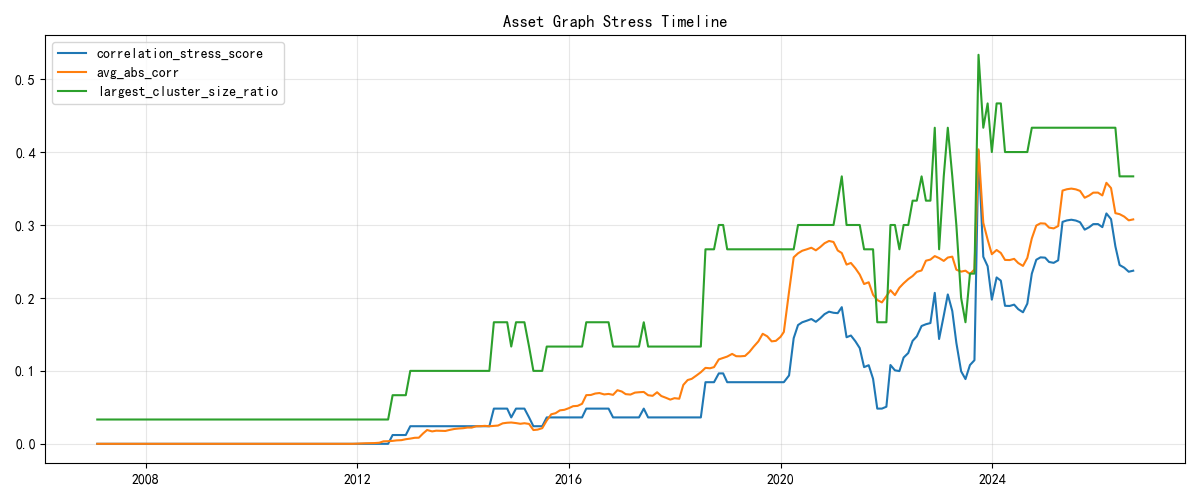
\includegraphics[width=0.84\textwidth]{asset_graph_stress_timeline.png}
    \caption{资产池跨类别相关结构}
    \label{fig:asset_graph}
  \end{figure}
}{}

相关结构图只作为历史描述，不直接生成主模型权重。主模型按调仓日前窗口估计风险，并通过凸目标和剩余约束生成组合。

\subsection{样本构造与预处理}
本文使用经复权处理后的可比价格序列，并据此计算相邻交易日收益率，同时对不同 ETF 的交易日进行对齐。保留真实极端收益，不使用全样本均值或标准差剔除异常收益。上市前缺失价格不作填补；若某 ETF 在再平衡日前的可用历史记录不足 60 个交易日，则不参与当期优化，满足门槛后方可进入可投资宇宙。价格数据通过 Tushare 接口获取，当前缓存中最早有效价格观测为 \dataFirstDate，最新缓存日期为 \dataLastDate；受限于各 ETF 上市时间，部分晚上市品种的有效样本更短。本文绩效评价区间自 \evalStartDate{} 起，至 \evalEndDate{} 止，将评价起点设定为该日期而非上市首日，是为保证多数资产在进入评价期前已积累足够的协方差估计历史窗口，避免初期样本不足带来的估计偏误。逐点时间宇宙过滤在每个再平衡日排除历史数据不足的 ETF，以避免前视信息泄露。部分资产如中证1000 ETF 上市时间较晚，因此其历史统计特征和模型参与频率与早上市 ETF 不完全一致，这一点在描述性统计与回测设计中已有体现。

\subsection{收益率、权重、交易成本与换手率定义}
设第 $i$ 个 ETF 在第 $t$ 日价格为 $P_{i,t}$，日收益率为：
\[
r_{i,t}=\frac{P_{i,t}}{P_{i,t-1}}-1
\]
调仓后权重为 $w_t$，调仓前经收益漂移后的权重为 $w_{t-1}^{+}$，组合毛收益为：
\[
r_{p,t}^{gross}=w_{t-1}^{T}r_t
\]
第 $t$ 个调仓日换手率定义为：
\[
TO_t=\sum_i |w_{i,t}-w_{i,t-1}^{+}|
\]
若单位交易成本率为 $c$，则交易成本为 $TC_t=c\cdot TO_t$，组合净收益为 $r_{p,t}^{net}=r_{p,t}^{gross}-TC_t$。本文默认交易成本为 3 bps，在结果中区分毛收益和净收益。该处理未覆盖冲击成本、买卖价差和申赎费用。

\subsection{组合约束与调仓规则}
主模型为多头且权重和为 1，不加杠杆。每周最后一个实际交易日调仓，节假日导致的缺失星期五由该周最后实际交易日替代。现金组与单资产集中度上限取消，其他组别边界和换手约束保留。期末不完整周沿用现有交易日历分组规则。

\subsection{评价指标体系}
累计净值为 $NAV_t=\prod_{s\leq t}(1+r_{p,s}^{net})$。主口径令 $r_{f,d}=0$，夏普与 Sortino 分别使用净收益标准差和下行均方根，按 243 日年化。机会成本诊断另令 $r_{f,d}=(1+y_{m-1})^{1/243}-1$，其中 $y_{m-1}$ 为上月最后有效的 1 年期中债国债收益率\cite{chinabond2026}。改变无风险利率只改变比率分子，不改变权重、收益或回撤。最大回撤定义为：
\[
MDD=\min_t\left(\frac{NAV_t}{\max_{s\leq t}NAV_s}-1\right)
\]
Calmar 比率为净年化收益除以最大回撤绝对值。平均月度换手率衡量组合执行稳定性。95\% 日度 CVaR 衡量历史日度损失超过 95\% 分位后的平均损失，是尾部风险诊断指标，不是未来极端损失预测。

\subsection{回测流程与无前视设计}
每次调仓先确定严格早于调仓日的历史窗口，再估计风险输入并求解目标权重。沿用项目记账规则，目标权重乘以当日收益并扣除换手成本，随后更新漂移权重；这属于日频回测执行约定，不是逐笔成交模拟。每次求解记录信息截止日，检查其早于交易日。评价期共 \primaryObservations{} 个日收益观察与 \primaryRebalances{} 个周频调仓点。逐期数据可得性检查不能消除规格事后选择带来的偏差。

无前视设计的时序实现可从代码层面加以说明。设第 $T$ 个月末为调仓日，协方差矩阵与风险预算估计所使用的收益率序列严格截止于 $T-1$ 日，即 $T$ 日当日价格（当日收益率 $r_T$）不进入本期估计窗口。$T$ 日优化求解完成后所得权重 $w_T$ 从 $T+1$ 日起生效，组合净值依据 $T+1$ 日及之后实现的收益率 $r_{T+1}, r_{T+2}, \ldots$ 进行计算。对于上市时间较短的主池 ETF（如中证2000、能源化工期货 ETF），可投资宇宙的纳入判断仅依赖截至 $T-1$ 日已观测到的历史记录：若有效观察不足 60 日，则在 $T$ 日调仓中排除。六支候选 ETF 则在整个回测中固定隔离。上述时序规则在回测引擎的数据切片逻辑中逐日强制执行，是保证无前视设计在实现层面不发生信息泄露的关键环节。

\subsection{可靠性与诊断层}
诊断层记录求解器状态、协方差条件数、半正定修复和逐期可投资宇宙。主模型评价期的 \primaryRebalances{} 个再平衡点均核查信息截止时间、权重预算、有效上限与交易成本。求解成功只说明数值问题得到可接受解，不能消除估计误差或事后规格选择偏差。具体最大违反量和复现容差见主模型审计文件。

\section{实证结果分析}
\subsection{主模型与核心对照}
表 \ref{tab:core_perf} 使用相同评价日期、零无风险利率与成本口径。主模型采用周频，其余模型为月频。主模型身份是研究定位，不表示其夏普或绝对收益在所有对照中最高。
\begin{table}[htbp]
\centering\small
\caption{主模型与核心对照}\label{tab:core_perf}
\resizebox{\textwidth}{!}{%
\begin{tabular}{lrrrrrr}
\toprule
模型 & 净年化收益 & 年化波动 & 夏普 & Sortino & 最大回撤 & 月均换手\\
\midrule
Improved Convex Adaptive Global RRP & \improvedNetReturn & \improvedVolatility & \improvedSharpe & \improvedSortino & \improvedMaxDD & \improvedMonthlyTurnover\\
Global RRP & \globalNetReturn & \globalVolatility & \globalSharpe & \globalSortino & \globalMaxDD & \globalMonthlyTurnover\\
Convex Adaptive Global RRP & \convexNetReturn & \convexVolatility & \convexSharpe & \convexSortino & \convexMaxDD & \convexMonthlyTurnover\\
HRP & \hrpNetReturn & \hrpVolatility & \hrpSharpe & \hrpSortino & \hrpMaxDD & \hrpMonthlyTurnover\\
HERC & \hercNetReturn & \hercVolatility & \hercSharpe & \hercSortino & \hercMaxDD & \hercMonthlyTurnover\\
Equal Weight & \equalWeightNetReturn & \equalWeightVolatility & \equalWeightSharpe & \equalWeightSortino & \equalWeightMaxDD & \equalWeightMonthlyTurnover\\
60/40 & \sixtyFortyNetReturn & \sixtyFortyVolatility & \sixtyFortySharpe & \sixtyFortySortino & \sixtyFortyMaxDD & \sixtyFortyMonthlyTurnover\\
\bottomrule
\end{tabular}}
\end{table}

主模型净年化收益为 \improvedNetReturn，年化波动为 \improvedVolatility，夏普为 \improvedSharpe，最大回撤为 \improvedMaxDD。零利率下，近现金模型可能具有较高比率，因此需要同时观察绝对收益、波动与资金集中度。所有结果均条件于当前样本与固定成本约定。

\subsection{净值、回撤与换手}
\figmaybe{convex_adaptive_nav_comparison.png}{主模型与对照累计净值}{fig:nav}
\figmaybe{convex_adaptive_drawdown_comparison.png}{主模型与对照回撤}{fig:drawdown}
主模型的较低波动伴随较高现金类 ETF 配置。最大回撤是实际历史路径的统计值，不由未启用的 CVaR 惩罚解释。频率与约束都会改变权重路径，主表跨模型比较不能隔离某一个因素的因果效应。
\figmaybe{convex_adaptive_turnover_comparison.png}{按自然月汇总的平均换手}{fig:turnover}
主模型的平均月度换手率为 \improvedMonthlyTurnover，调仓日历仍为周频。换手按交易前漂移权重与目标权重的 $L_1$ 距离计算，成本等于该距离乘以 3 bps。固定费率不包含实测价差、市场冲击与容量影响。

\subsection{现金集中度与尾部风险}
\figwide{primary_weights.png}{主模型权重路径}{fig:weight_path}
平均现金类 ETF 权重为 \primaryCashMean，最大值为 \primaryCashMax。取消现金上限并不等价于增加杠杆，也不保证风险来源充分分散。集中配置于低波动基金，是低组合波动和零利率夏普的重要解释。
\figmaybe{convex_adaptive_cvar_comparison.png}{核心模型历史尾部损失}{fig:cvar}
主表沿用历史尾均值统计以保证核心模型之间一致；约束实验采用分位点质量可拆分的精确经验 CVaR，与凸辅助变量形式一致。两者均以 95\% 为研究口径，未搜索置信水平。

\subsection{期末权重快照}
% Auto-generated by scripts/export_next_month_holdings.py
截至 2026-08-31 的模型输出对应 2026-09 持仓。
\begin{table}[H]
\centering
\scriptsize
\setlength{\tabcolsep}{3.2pt}
\caption{2026-09 Improved Convex Adaptive Global RRP 持仓}
\label{tab:next_month_holdings}
\begin{tabular}{llrllr}
\toprule
ETF & 代码 & 权重 & ETF & 代码 & 权重 \\
\midrule
日利ETF & 511880.SH & 30.00\% & 中证1000ETF & 512100.SH & 1.44\% \\
信用债ETF & 511030.SH & 10.01\% & 消费ETF & 159928.SZ & 1.25\% \\
5年国债ETF & 511010.SH & 7.70\% & 豆粕ETF & 159985.SZ & 0.82\% \\
10年国债ETF & 511260.SH & 6.64\% & 军工ETF & 512660.SH & 0.80\% \\
黄金ETF & 518880.SH & 4.70\% & 能源化工期货ETF & 159981.SZ & 0.58\% \\
纳指ETF & 159941.SZ & 3.72\% & 半导体ETF & 512480.SH & 0.57\% \\
标普500ETF & 513500.SH & 3.68\% & 日经225ETF & 513880.SH & 0.56\% \\
欧洲ETF & 513030.SH & 3.42\% & 煤炭ETF & 515220.SH & 0.51\% \\
原油ETF & 162411.SZ & 3.33\% & 中证2000ETF & 563300.SH & 0.51\% \\
恒生ETF & 159920.SZ & 3.30\% & 科创50ETF & 588000.SH & 0.50\% \\
红利ETF & 510880.SH & 3.29\% & 人工智能ETF & 159819.SZ & 0.50\% \\
沪深300ETF & 510300.SH & 3.10\% & 可转债ETF & 511380.SH & 0.49\% \\
创业板ETF & 159915.SZ & 2.98\% & 有色金属期货ETF & 159980.SZ & 0.48\% \\
中证500ETF & 510500.SH & 2.52\% & 证券ETF & 512880.SH & 0.48\% \\
白银LOF & 161226.SZ & 1.67\% & 新能源ETF & 516160.SH & 0.45\% \\
\bottomrule
\end{tabular}
\end{table}

期末持仓展示模型实际暴露。它不表示下一自然月保持不变，周频模型将在后续再平衡点使用新历史窗口求解。

\section{约束诊断与研究边界}
\subsection{集中度和风险控制消融}
约束实验使用共同日期和未剔除极端值的收益。月度与周频集中度约束对照保留现金 30\%、单资产 40\% 上限。仅取消现金上限时仍受单资产上限限制；只有同时取消两项上限，现金权重才能进一步上升。
\begin{table}[htbp]
\centering\scriptsize
\caption{固定约束实验与利率口径对照}
\resizebox{\textwidth}{!}{\begin{tabular}{lrrrr}
\toprule
生效年 & $\lambda_{v,t}$ & $\lambda_{r,t}$ & 验证夏普 & 标准误集合\\\midrule
2017 & 6.858e-12 & 16.54 & 1.467 & 9/9\\
2018 & 0.1402 & 8.826 & 1.630 & 9/9\\
2019 & 0.08214 & 24.72 & 0.026 & 9/9\\
2020 & 0.1012 & 9.385 & 3.433 & 9/9\\
2021 & 0.1181 & 2.936 & 1.629 & 9/9\\
2022 & 0.08515 & 2.01 & 2.051 & 9/9\\
2023 & 0.1336 & 8.52 & 0.280 & 9/9\\
2024 & 0.2022 & 11.52 & 2.796 & 9/9\\
2025 & 0.1931 & 15.49 & 2.547 & 9/9\\
2026 & 0.1574 & 3.793 & 2.207 & 9/9\\
\bottomrule
\end{tabular}}
\end{table}
无风险利率设为零时，主模型夏普达到 \improvedSharpe；同一组合以中债利率为机会成本时夏普为 \primaryChinaBondSharpe。这是统计口径差异，不是额外投资收益。取消单资产上限但保留现金组上限时，该约束组合仍限制现金集中，不能将其解释为完全放开现金配置。

相对 CVaR 实验先求基准可行组合，再使用该组合场景 CVaR 作为候选上限。由于基准本来就是原目标的最优解，新约束在精确求解下不要求改变权重。微小权重或夏普差异可能来自数值容差，不能作为独立改善证据。Ledoit--Wolf 实验由历史数据估计收缩强度，不继承消融的全样本赢家。

\subsection{自然年结果}
\begin{table}[htbp]
\centering\small
\caption{主模型分自然年绩效}
\begin{tabular}{lrrrr}
\toprule
年份 & 净年化收益 & 年化波动 & 夏普 & 最大回撤\\\midrule
2018 & 0.06\% & 3.79\% & 0.034 & -5.04\%\\
2019 & 14.29\% & 8.11\% & 1.696 & -4.30\%\\
2020 & 22.20\% & 10.86\% & 1.908 & -7.16\%\\
2021 & 9.24\% & 6.12\% & 1.481 & -3.37\%\\
2022 & -1.58\% & 3.95\% & -0.384 & -3.19\%\\
2023 & 3.93\% & 3.44\% & 1.144 & -1.76\%\\
2024 & 12.51\% & 10.86\% & 1.144 & -6.95\%\\
2025 & 16.30\% & 8.67\% & 1.793 & -3.34\%\\
2026 & 22.82\% & 8.35\% & 2.519 & -4.69\%\\
\bottomrule
\end{tabular}
\end{table}
每个自然年单独计算净值、波动与回撤；年度最大回撤不等于跨年连续路径回撤。2026 年仅覆盖至 \evalEndDate，年化指标不代表完整年度已实现收益。年度之间的差异说明全期高比率不保证每个阶段达到同一目标。

\subsection{频率敏感性}
频率实验保留主模型参数及冻结候选日历，只改变周、双周、月、季度再平衡规则。它与保留集中度约束的周频基准不是同一实验。
% Auto-generated by scripts/generate_thesis_numbers.py
% Source: results/tables/rebalance_frequency_sensitivity.csv
% Do not edit by hand.
\begin{table}[H]
\centering
\small
\caption{调仓频率敏感性检验（固定 Improved Convex Adaptive Global RRP 参数）}
\label{tab:rebalance_frequency_sensitivity}
\begin{tabular}{lrrrrrr}
\toprule
调仓频率 & 调仓次数 & 净年化收益 & Sharpe & 最大回撤 & 月均换手 & 求解器回退率 \\
\midrule
周度 & 439 & 5.38\% & 1.118 & -3.65\% & 3.06\% & 0.00\% \\
双周 & 219 & 5.36\% & 1.109 & -3.65\% & 2.54\% & 0.00\% \\
月度 & 103 & 5.60\% & 1.186 & -3.81\% & 1.96\% & 0.00\% \\
季度 & 35 & 5.26\% & 1.042 & -3.77\% & 1.69\% & 0.00\% \\
\bottomrule
\multicolumn{7}{l}{\footnotesize 仅改变调仓日历，不重新选择候选参数；月均换手按评价窗口内总换手除以月数计算。} \\
\end{tabular}
\end{table}

\figmaybe{rebalance_frequency_sensitivity.png}{主模型参数下的调仓频率比较}{fig:rebalance_frequency_sensitivity}
周频为当前指定主模型配置，表中事后排名仅作描述，不据此继续扩大频率搜索。

\subsection{可重复性与统计解释}
主模型在 \primaryObservations{} 个共同交易日上复现了获批研究路径。逐期检查包括权重归一、成本一致性、交易前漂移权重、信息截止时间、实际组上限、求解状态与最大约束违反量。诊断结果保存在主模型发布审计文件中。

这些检查验证实现与记账，不检验模型选择的统计显著性。主模型规格经历史实验后确定，不能将冻结日历视为对最终规格的独立样本外验证。历史 CSCV、PBO、参数扰动与自助检验属于其各自记录的模型版本，未作为当前规格的有效性证明。未来验证应预先冻结规格并使用新增数据，不反复追求全样本阈值。

\section{结论与展望}
\subsection{主要结论}
主模型以风险预算参考和凸跟踪目标生成多头周频组合，取消现金与单资产集中度上限，保留换手和非现金组别约束。其净年化收益为 \improvedNetReturn，波动为 \improvedVolatility，零利率夏普为 \improvedSharpe，最大回撤为 \improvedMaxDD。平均现金类 ETF 权重为 \primaryCashMean，是解释结果不可省略的配置特征。

Global RRP、基础凸模型、层次化模型与静态基准用于对照。主模型不是所有指标的最优者，零利率比率也不等同于相对国债的超额收益效率。约束诊断将结构变化与口径变化分开，能够解释哪些配置实际上改变权重。

\subsection{研究边界}
研究采用固定 3 bps 成本，不包含容量、价差与冲击估计。主模型未显式建模负债、久期缺口与资本占用，不能直接据此认定适用于保险资产负债管理。部分 ETF 上市较晚，前向价格填充也不能完全表达停牌期间的实际可交易性。执行时序为日频研究约定，实际成交需要独立验证。

规格选择使用了历史实验结果。下一步应冻结参数、资产池和评价口径，以新增数据验证稳定性；不得将这组事后结果表述为未来收益承诺。

\clearpage
\appendix
\section{主模型配置与复现}
主模型配置来源于 \texttt{primary\_model\_configuration.json}，代码入口为 \texttt{scripts/run\_primary\_publication\_pipeline.py}。每次完整运行先刷新行情与利率，再重算核心模型和频率对照、生成论文数字、编译论文及答辩材料并清理临时文件。

单资产上限 1 是多头预算的冗余边界。现金没有组上限，其余组别上限保留。CVaR 扩展使用 95\% 场景损失，主模型相应系数为零。所有继承参数均应视为可复现研究约定，不宣称通过市场数据唯一识别。

\section{历史候选记录}
既有 36 组候选和季度日历仅供原研究追溯。当前主模型是冻结日历上的统一结构变换，不重新通过全样本候选分数选择参数。历史文件不作为当前主模型过拟合概率或统计显著性的估计。

\bibliographystyle{gbt7714-numeric}
\bibliography{references}

\clearpage
\phantomsection
\addcontentsline{toc}{section}{致谢}
\section*{致谢}

本文得以完成，首先要感谢指导老师王磊教授。从选题方向的确定、研究框架的搭建，到实证方法的细化与论文的反复修改，王老师在每一个关键节点都给予了耐心细致的指导与建设性意见，使我对量化资产配置领域的认识不断深化。王老师严谨的学术态度和对学生的真诚关怀，是我在整个研究过程中最重要的精神支撑。

感谢特拉华数据科学学院和金融数学专业的各位任课老师，你们在数学基础、金融理论与编程实践方面的悉心教导，为本文的研究工作打下了坚实的基础。感谢同门同学在学习与讨论中给予的启发与帮助。

最后，衷心感谢父母多年来的理解、支持与付出。你们的鼓励始终是我前行最大的动力。

\end{document}
